\section{Deterministic Variational Approach}
There are two main parts for computing the reconstruction term: propagation of distributions through activations to compute $\tilde{q}(\mathbf{a}^L)$, and evaluation of unparameterized log-likelihood $\mathcal{L}$. In Fig~\ref{fig:feed_arch} we can see the general architecture used to accomplish these tasks.

\begin{figure}[H]
\centering
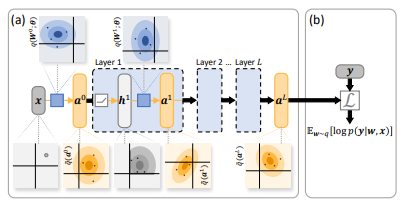
\includegraphics[scale=.5]{fig/dvi-architect-p1.png}
\caption{Feed-forward architecture for reconstruction term computation.}
\label{fig:feed_arch}
\end{figure}

\noindent\textbf{Moment Propagation.} \\
We can consider the model, $\mathcal{M}$, as a set of layers each containing an non-linear and affine transformation,
$$
\mathcal{M} := \{(\bm{h}^l,\bm{a}^l): \bm{h}^l = f(\bm{a}^{l-1}), \bm{a}^l = \bm{h}^l\bm{W}^l + \bm{b}^l\}_{l=1}^{\mathbb{N}}
$$

where $\{\bm{W},\bm{b}\}\subset\bm{\omega}$ are random variables representing the weights and are assumed independent per layer. $\bm{a}^l$ is argued to be Gaussian under the Central Limit Theorem given a sufficiently large latent space and finite $1^{st}$ and $2^{nd}$ moment since it is formulated as the linear combination of the elements of $\bm{h}^l$. Given that $\bm{a}^l$ is Gaussian we can appoximate the $1^{st}$ and $2^{nd}$ moment,

\begin{equation}
\langle a_i\rangle = \langle h_j\rangle\langle W_{ji}\rangle + \langle b_i\rangle
\end{equation}
$$
\text{Cov}(a_i,a_k) = 
$$
\begin{equation}
\langle h_jh_l\rangle\text{Cov}(W_{ji},W_{lk})+ \langle W_{ji}\rangle\text{Cov}(h_j,h_l)\langle W_{lk}\rangle + \text{Cov}(b_i,b_k)
\end{equation}

where $\langle a_i\rangle := \mathbb{E}_{q}[a_i]$ and $h_jW_{ji} = \sum_{j=1}^nh_jW_{ji}$ is called Einstein notation. To reduce approximation, gaussian distributions are considered for the mean and covariance of the weights so that all that is left determine are the moments $\langle h_j\rangle$ and $\langle h_jh_l\rangle$

\begin{equation}
\langle h_j\rangle \propto \int f(\alpha_j)\exp\bigg[-\frac{(\alpha_j-\langle a_j^{l-1}\rangle)^2}{2\Sigma_{jj}^{l-1}}\bigg]d\alpha_j
\end{equation}

\begin{equation}
\langle h_jh_l\rangle \propto \int f(\alpha_j)f(\alpha_l)\exp\bigg[-\frac{1}{2}\zeta^T\Lambda^{-1}\zeta\bigg]d\alpha_jd\alpha_l
\end{equation}

$$
\zeta = \begin{pmatrix} \alpha_j - \langle a_j^{l-1}\rangle\\ \alpha_l - \langle a_l^{l-1}\rangle\\\end{pmatrix}
$$

$$
\Lambda = \begin{pmatrix} \Sigma_{jj}^{l-1} & \Sigma_{jl}^{l-1}\\ \Sigma_{lj}^{l-1} & \Sigma_{ll}^{l-1}\\\end{pmatrix}
$$

 Closed form solutions exist for (4) when considering Heaviside or ReLU non-linearity for $f$. For (5), we can approximate the moment through,

\begin{equation}
\langle h_jh_l\rangle = S_{jl}^{l-1}\bigg\{A(\mu_j^{l-1},\mu_{l}^{l-1},\rho_{jl}^{l-1})+\exp[-Q(\mu_j^{l-1},\mu_l^{l-1},\rho_{jl}^{l-1})]\bigg\}
\end{equation}

where the key idea is that the asymptotes $A$ of the non-linearities as well as the residuals $Q$ in the form of a polynomial provide a good first order approximation of the moment. Fig~\ref{fig:approx} provides a visual representation of this process. Due to CLT these approximations provide sufficient information for us to explicitly determine $\tilde{q}(\bm{a}^L)$ through sequential distribution propagation.

\begin{figure}[H]
\centering
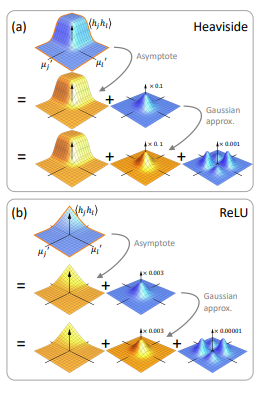
\includegraphics[scale=.5]{fig/activations.png}
\caption{Model activation function approximation.}
\label{fig:approx}
\end{figure}

\noindent\textbf{Log-Likelihood Evaluation.} \\
We can evaluate the expected log-likelihood $\mathbb{E}_{\bm{\omega}\sim q}\big[\log p(y \mid \bm{x},\bm{\omega})\big]$ through directly evaluating $\mathbb{E}_{\bm{a}^L\sim q(\bm{a}^L)}\big[\log p(y \mid \bm{a}^L)\big]$ since $q(y \mid \bm{a}^L)$ is a parameter free transformation.

\section{Empirical Bayes for Variational BNNs}

Considering a $d$-dimensional Gaussian prior, $p(\bm{\omega}) = \mathcal{N}(\mu_p,\Sigma_p)$, and variational distribution, $q = \mathcal{N}(\mu_q,\Sigma_q)$, the KL divergence has the form,

\begin{equation}
\frac{1}{2}\bigg[\log\frac{\det(\Sigma_p)}{\det(\Sigma_q)} - d + \text{tr}(\Sigma_p^{-1}\Sigma_q) + (\mu_p - \mu_q)^T\Sigma_p^{-1}(\mu_p - \mu_q)\bigg]
\end{equation}

Rather than using this directly the authors propose conditioning the prior on a hyper-parameter $\bm{s}$ such that $\bm{\omega}\sim p(\bm{\omega}\mid\bm{s}); \bm{s} \sim p(\bm{s})$, where $\bm{s}$ is distributed according to a inverse gamma distribution and acts as a conjugate prior for the diagonal gaussian variance. Further through partioning the weights $\bm{\omega}$ into sets $\{\lambda\}$ such that an element $s_\lambda$ of $\bm{s}$ can be assigned to each set,
$$
s_\lambda \sim \text{Inv-Gamma}(\alpha,\beta), \quad w_i^\lambda \sim \mathcal{N}(0,s_\lambda) 
$$
we can consider solving the MAP optimization problem for the KL divergence,

$$
s^*_\lambda = \argmin_{s_\lambda} KL\bigg[q(\bm{\omega};\bm{\theta})||p(\bm{\omega}^\lambda\mid s_\lambda) - \log p(s_\lambda)\bigg]
$$

This leads to the closed-form solution,
$$
s^*_\lambda = \frac{\text{tr}(\Sigma_q^\lambda+\mu_q^\lambda(\mu_q^\lambda)^T)+2\beta}{\Omega_\lambda + 2\alpha + 2}
$$

where $\Omega_\lambda := |\lambda|$. We can then use $s^*_\lambda$ to determine the diagonal entries of $\Sigma_p$ and solve (1).

\begin{figure}[H]
\centering
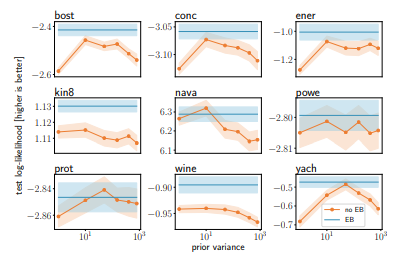
\includegraphics[scale=.5]{fig/empirical-bayes.png}
\caption{Test Log-likelihood with tuned prior (orange) and EB (blue).}
\label{fig:emp_bayes}
\end{figure}
